\documentclass{article}


\usepackage{longtable}
\usepackage[margin=1in]{geometry}
\usepackage[section]{placeins}
\usepackage{cite}

\title{Improving Day Ahead Electricity Load Forecasts with Google Trends}
\author{Cameron Mulder\\ James Woods}

% \date{}
 

\usepackage{Sweave}
\begin{document}
\maketitle
\setkeys{Gin}{width=0.7\textwidth}


\begin{abstract}
Modern short term load forecasting has grown in analytically complexity and sophistication.  Day ahead forecasts now commonly use neural nets, Monte Carlo simulations and a wealth of historical data.  What they have not done is fully captured the sentiment and intentions of the people using the electricity.  This paper introduces Google Trend data, a summary of Google searches, as a way of capturing this sentiment and refining forecasts.  We show with drop all forward cross validation that this amendment decreases forecast uncertainty by approximately 5\% when compared to a statistically adjusted forecast and by over 50\% when compared to raw forecasts.
\end{abstract}

\Sconcordance{concordance:DraftPaper.tex:DraftPaper.Rnw:%
1 14 1 1 0 13 1 1 9 13 1 1 11 7 1 1 8 1 2 7 1 1 8 1 2 18 1 1 11 1 3 9 1 %
1 11 1 3 19 1 1 23 2 1 1 9 5 1 1 9 1 2 5 1 1 15 7 1 1 25 1 1 1 5 35 0 1 %
2 18 1 1 13 42 0 1 2 9 1 1 3 32 0 1 1 32 0 1 1 32 0 1 1 32 0 1 1 32 0 1 %
1 32 0 1 2 1 1 1 2 32 0 1 1 32 0 1 1 32 0 1 1 32 0 1 1 32 0 1 1 32 0 1 %
3 1 1 1 3 32 0 1 1 32 0 1 1 32 0 1 1 32 0 1 1 32 0 1 1 32 0 1 2 2 1 1 3 %
32 0 1 1 32 0 1 1 32 0 1 1 32 0 1 1 32 0 1 1 32 0 1 7 5 1}


\section{Introduction}



\begin{enumerate}
  \item Intro to short term load forecasting.
  \item Why crowd sourced, non technical,  information could be useful.
  \item Google trends is the summation of Google searches.
  \item Outline of paper
\end{enumerate}


\section{Data Sources}

  \subsection{PJM Load Forecasts and Actuals}
  
  





\begin{figure}
\begin{center}
\caption{Confidence Intervals for Intercept Statistically Adjusted Models (95\%)}
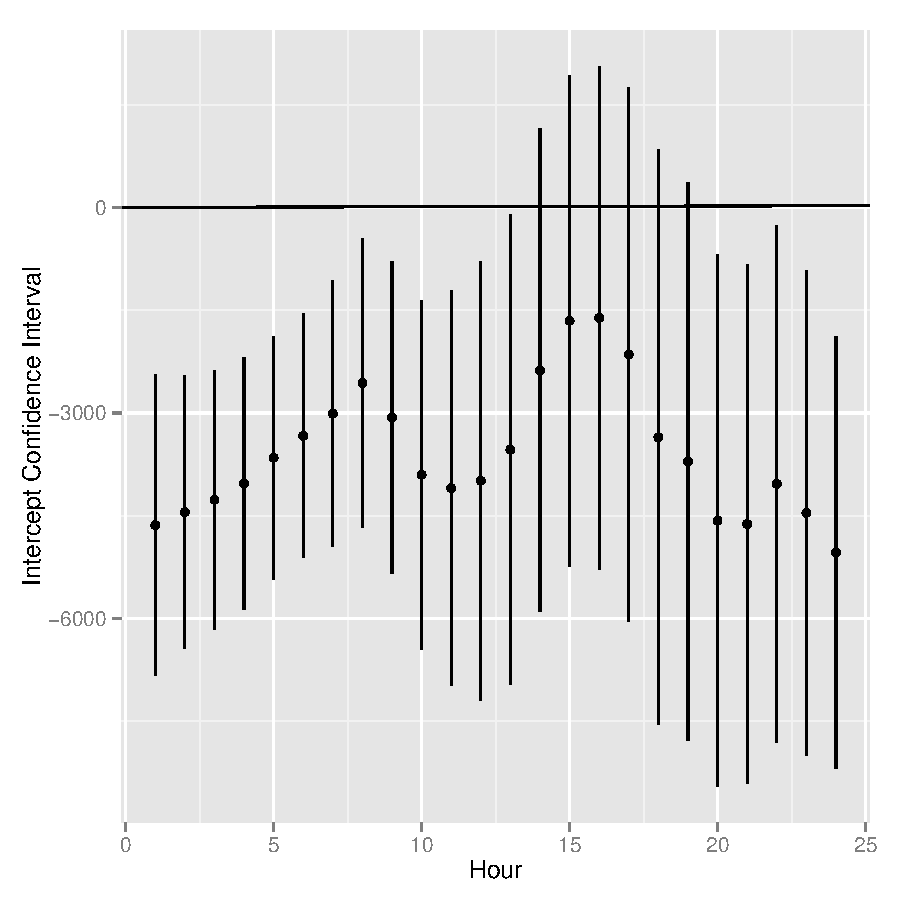
\includegraphics{DraftPaper-003}
\end{center}
\end{figure}



\begin{figure}
\begin{center}
\caption{Confidence Intervals for Co-Movement Statistically Adjusted Models (95\%)}
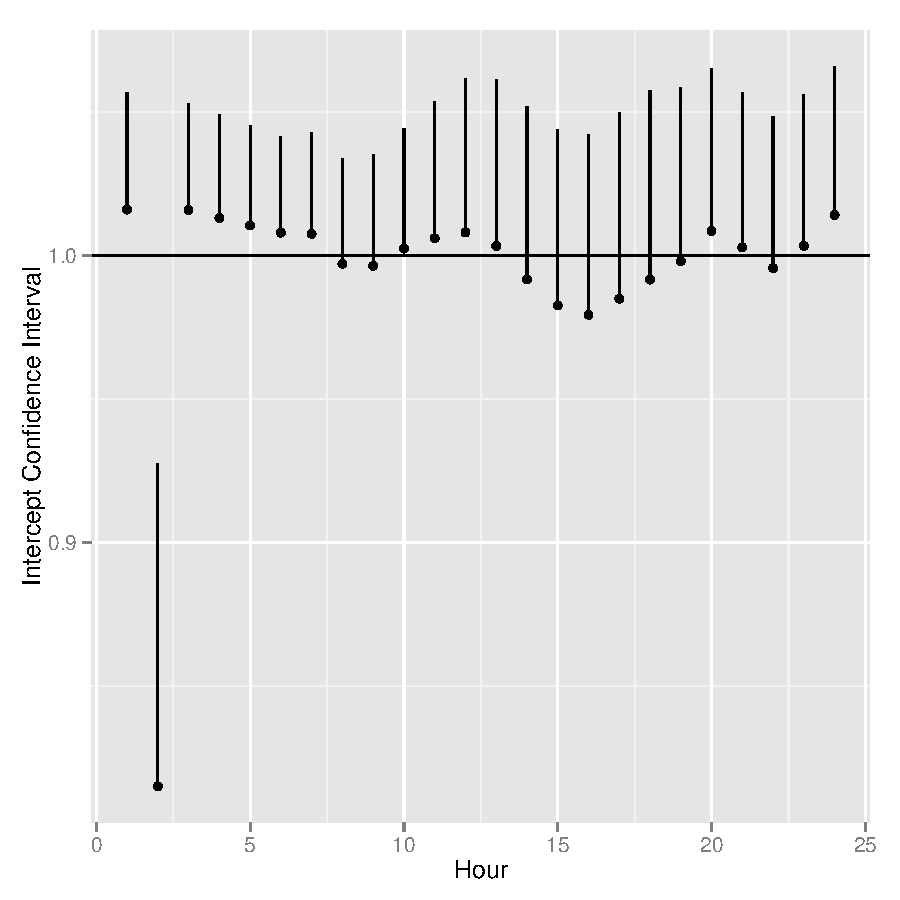
\includegraphics{DraftPaper-004}
\end{center}
\end{figure}




    \begin{enumerate}
      \item Data sources.
      \item Documentation of forecasting.
      \item Forecast bias
      \item Statistically adjusted forecasts.
      \item Note that almost all hours are biased and that co-movements are good for peak hours
    \end{enumerate}

  \subsection{Google Trends}

\begin{figure}
\begin{center}
\caption{State Weather Trends Indexes Over Time}
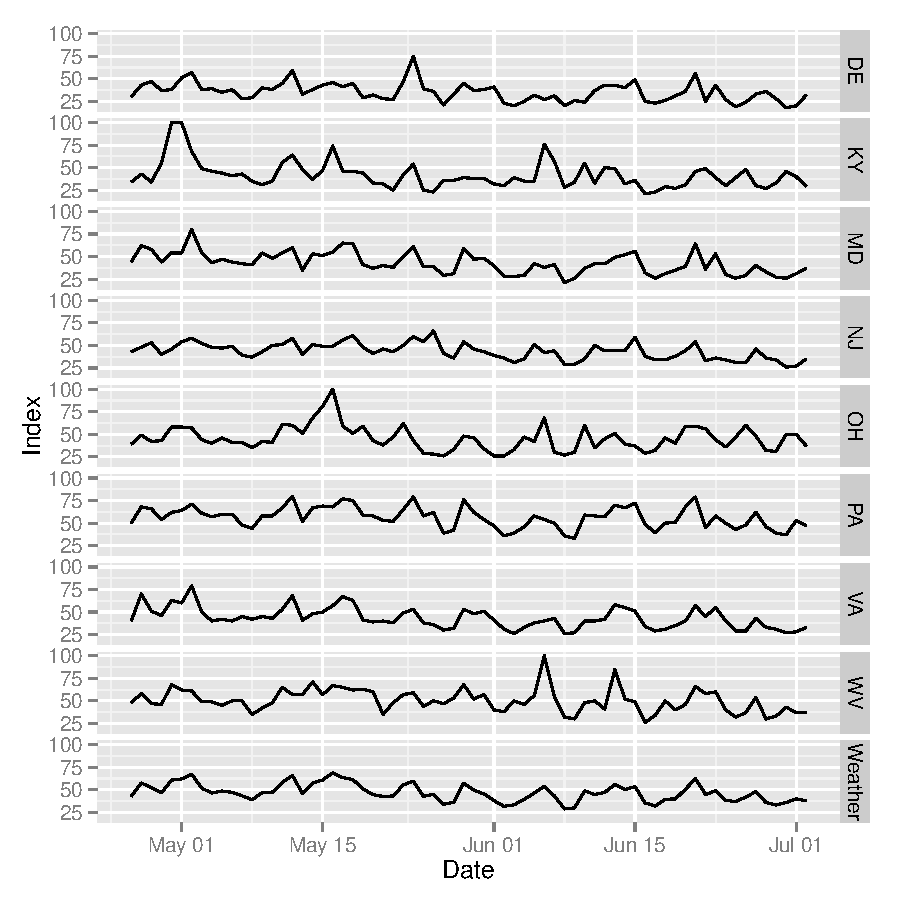
\includegraphics{DraftPaper-005}
\end{center}
\end{figure}





\begin{figure}
\begin{center}
\caption{Trends Indexes Over Time}
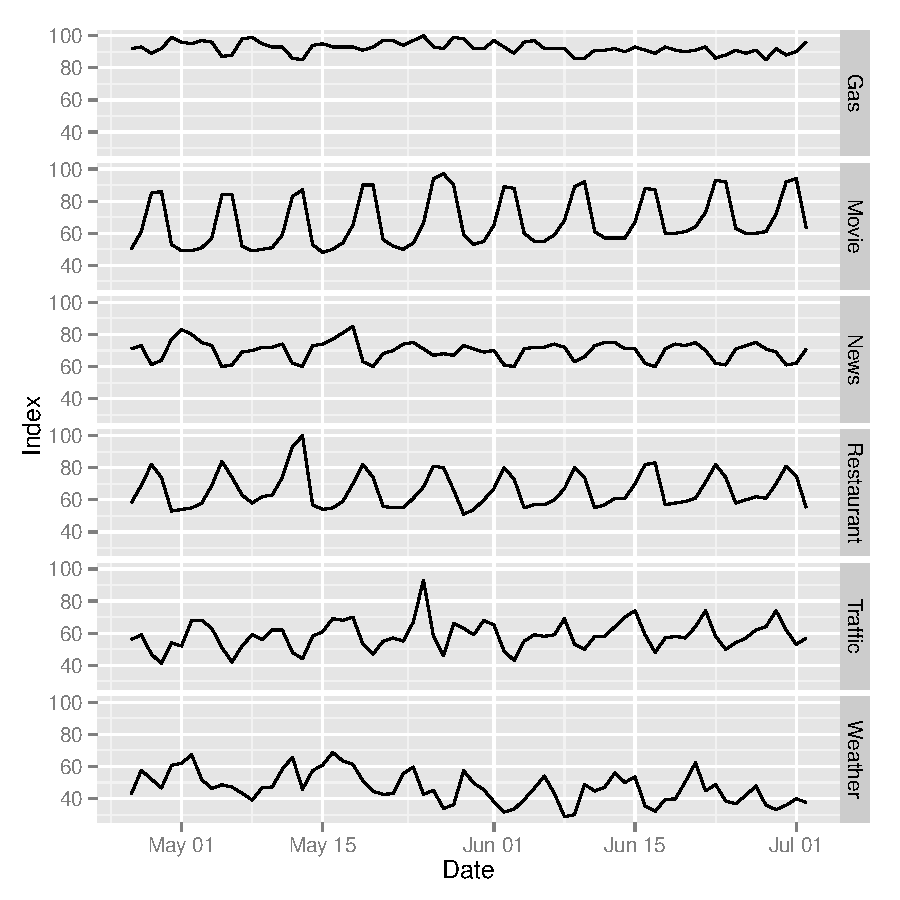
\includegraphics{DraftPaper-006}
\end{center}
\end{figure}



    \begin{enumerate}
      \item Where to get the data
      \item Limitations
      \item Forming a population weighted index.
      \item Other common searches that will be used as counter examples.
    \end{enumerate}

\section{Post Forecast Addition of Google Trends Data}

  \begin{enumerate}
    \item Simple hourly models with Trends.
    \item Gross comparison with actual forecast and statistically adjusted forecasts.
    \item Why this is insufficient.
  \end{enumerate}







\begin{figure}
\begin{center}
\caption{Confidence Intervals for ``Weather'' in Trends Models (95\%)}
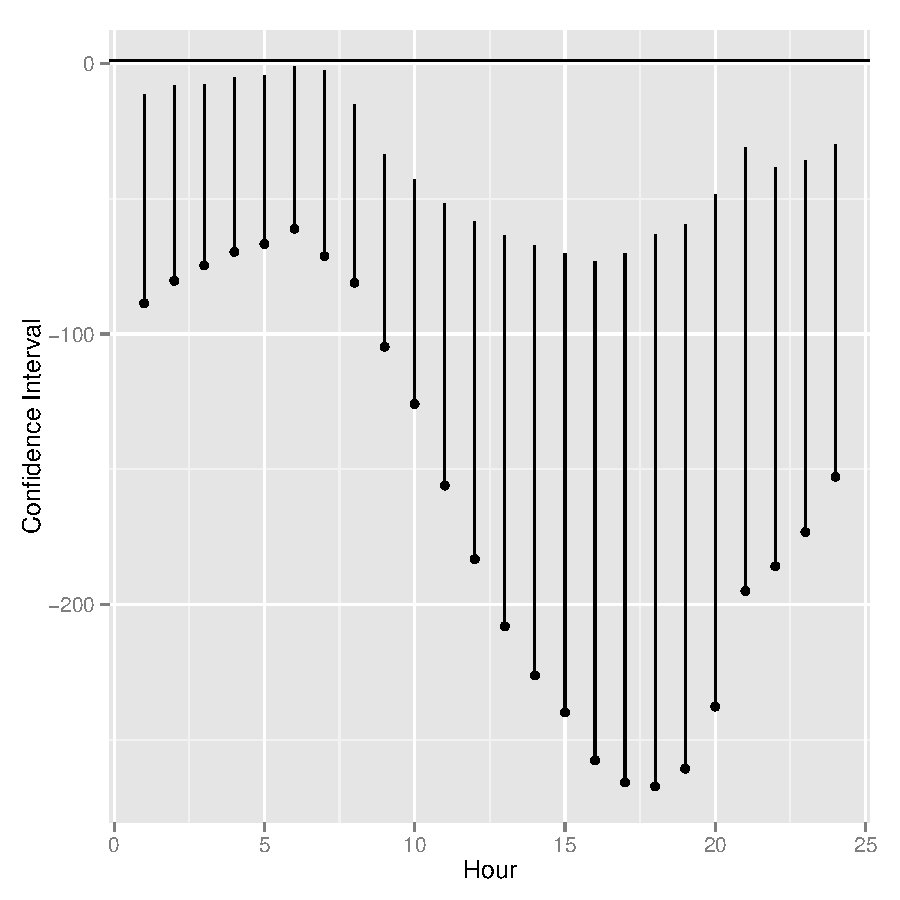
\includegraphics{DraftPaper-009}
\end{center}
\end{figure}



  






  \subsection{Drop Forward Cross-validation}


  
% Table created by stargazer v.5.1 by Marek Hlavac, Harvard University. E-mail: hlavac at fas.harvard.edu
% Date and time: Tue, Aug 05, 2014 - 12:02:43 PM
\begin{table}[!htbp] \centering 
  \caption{Improvement in Forecasts Relative to Gross,  Statistically Adjusted, Drop Forward CV (Percent)} 
  \label{} 
\begin{tabular}{@{\extracolsep{5pt}} cccc} 
\\[-1.8ex]\hline 
\hline \\[-1.8ex] 
Hour & Direct & Statistically Adjusted (Raw) & Statistically Adjusted (CV) \\ 
\hline \\[-1.8ex] 
$1$ & $$ & $6.832$ & $4.386$ \\ 
$2$ & $$ & $7.018$ & $4.279$ \\ 
$3$ & $$ & $6.872$ & $4.672$ \\ 
$4$ & $$ & $6.553$ & $4.148$ \\ 
$5$ & $$ & $6.630$ & $3.965$ \\ 
$6$ & $$ & $6.871$ & $4.153$ \\ 
$7$ & $$ & $7.850$ & $4.299$ \\ 
$8$ & $$ & $9.913$ & $7.156$ \\ 
$9$ & $$ & $10.652$ & $11.218$ \\ 
$10$ & $$ & $9.261$ & $11.145$ \\ 
$11$ & $$ & $7.892$ & $10.028$ \\ 
$12$ & $$ & $6.713$ & $8.147$ \\ 
$13$ & $$ & $6.403$ & $6.824$ \\ 
$14$ & $$ & $6.160$ & $6.077$ \\ 
$15$ & $$ & $6.027$ & $5.374$ \\ 
$16$ & $$ & $5.915$ & $5.427$ \\ 
$17$ & $$ & $5.617$ & $4.946$ \\ 
$18$ & $$ & $4.961$ & $4.369$ \\ 
$19$ & $$ & $4.750$ & $4.365$ \\ 
$20$ & $$ & $4.872$ & $2.099$ \\ 
$21$ & $$ & $5.694$ & $1.257$ \\ 
$22$ & $$ & $6.267$ & $3.485$ \\ 
$23$ & $$ & $5.793$ & $3.631$ \\ 
$24$ & $$ & $5.160$ & $2.972$ \\ 
\hline \\[-1.8ex] 
\end{tabular} 
\end{table}   
  
  
    \begin{enumerate}
      \item Cross validation concepts.
      \item Why drop forward cross validation is the right concept.
      \item Comparison of drop forward statistically adjusted and Trends adjusted with gross comparisons.
      \item Reiteration that comparison with raw forecasts is a slam dunk.
    \end{enumerate}
    
  \subsection{Counter-factual Test with Other Common Google Searches}
  
  
  
    \begin{enumerate}
      \item Comparison with: news, recipe, traffic, gas.
      \item Note that some of them kinda work.
    \end{enumerate}
    
% Table created by stargazer v.5.1 by Marek Hlavac, Harvard University. E-mail: hlavac at fas.harvard.edu
% Date and time: Tue, Aug 05, 2014 - 12:02:44 PM
\begin{table}[!htbp] \centering 
  \caption{Alternate Google Search Models for Hour 19} 
  \label{} 
\begin{tabular}{@{\extracolsep{5pt}}lccccc} 
\\[-1.8ex]\hline 
\hline \\[-1.8ex] 
 & \multicolumn{5}{c}{Hour 19 Load} \\ 
\cline{2-6} 
 & News & Gas & Traffic & Restaurant & Movie \\ 
\\[-1.8ex] & (1) & (2) & (3) & (4) & (5)\\ 
\hline \\[-1.8ex] 
 F19 & 0.987$^{***}$ & 1.001$^{***}$ & 1.004$^{***}$ & 0.985$^{***}$ & 0.974$^{***}$ \\ 
  & (0.032) & (0.032) & (0.032) & (0.031) & (0.032) \\ 
  & & & & & \\ 
 NewsTrends & $-$109.127$^{**}$ &  &  &  &  \\ 
  & (54.369) &  &  &  &  \\ 
  & & & & & \\ 
 GasTrends &  & $-$100.782 &  &  &  \\ 
  &  & (88.731) &  &  &  \\ 
  & & & & & \\ 
 TrafficTrends &  &  & $-$19.657 &  &  \\ 
  &  &  & (31.495) &  &  \\ 
  & & & & & \\ 
 RestaurantTrends &  &  &  & 84.677$^{**}$ &  \\ 
  &  &  &  & (33.519) &  \\ 
  & & & & & \\ 
 MovieTrends &  &  &  &  & 61.023$^{**}$ \\ 
  &  &  &  &  & (24.515) \\ 
  & & & & & \\ 
 Constant & 8,950.203 & 9,010.925 & 581.895 & $-$4,227.396 & $-$1,637.760 \\ 
  & (5,944.583) & (9,658.220) & (4,357.965) & (3,326.853) & (3,064.397) \\ 
  & & & & & \\ 
\hline \\[-1.8ex] 
Observations & 88 & 88 & 88 & 88 & 88 \\ 
Log Likelihood & $-$811.334 & $-$812.185 & $-$813.666 & $-$810.691 & $-$811.109 \\ 
Akaike Inf. Crit. & 1,632.669 & 1,634.370 & 1,637.332 & 1,631.383 & 1,632.219 \\ 
Bayesian Inf. Crit. & 1,644.882 & 1,646.584 & 1,649.546 & 1,643.596 & 1,644.432 \\ 
\hline 
\hline \\[-1.8ex] 
\textit{Note:}  & \multicolumn{5}{r}{$^{*}$p$<$0.1; $^{**}$p$<$0.05; $^{***}$p$<$0.01} \\ 
\end{tabular} 
\end{table} 


\section{Summary and Conclusions}


\appendix

\section{Hourly Models with Weather Searches}

% Table created by stargazer v.5.1 by Marek Hlavac, Harvard University. E-mail: hlavac at fas.harvard.edu
% Date and time: Tue, Aug 05, 2014 - 12:02:44 PM
\begin{table}[!htbp] \centering 
  \caption{Hour 1} 
  \label{} 
\begin{tabular}{@{\extracolsep{5pt}}lc} 
\\[-1.8ex]\hline 
\hline \\[-1.8ex] 
 & \multicolumn{1}{c}{\textit{Dependent variable:}} \\ 
\cline{2-2} 
\\[-1.8ex] & Hour 1 \\ 
\hline \\[-1.8ex] 
 Forecast & 0.990$^{***}$ \\ 
  & (0.023) \\ 
  & \\ 
 Weather & $-$52.323$^{***}$ \\ 
  & (15.875) \\ 
  & \\ 
 Constant & 2,559.469 \\ 
  & (2,170.601) \\ 
  & \\ 
\hline \\[-1.8ex] 
Observations & 96 \\ 
Log Likelihood & $-$827.731 \\ 
Akaike Inf. Crit. & 1,665.461 \\ 
Bayesian Inf. Crit. & 1,678.124 \\ 
\hline 
\hline \\[-1.8ex] 
\textit{Note:}  & \multicolumn{1}{r}{$^{*}$p$<$0.1; $^{**}$p$<$0.05; $^{***}$p$<$0.01} \\ 
\end{tabular} 
\end{table} % Table created by stargazer v.5.1 by Marek Hlavac, Harvard University. E-mail: hlavac at fas.harvard.edu
% Date and time: Tue, Aug 05, 2014 - 12:02:44 PM
\begin{table}[!htbp] \centering 
  \caption{Hour 2} 
  \label{} 
\begin{tabular}{@{\extracolsep{5pt}}lc} 
\\[-1.8ex]\hline 
\hline \\[-1.8ex] 
 & \multicolumn{1}{c}{\textit{Dependent variable:}} \\ 
\cline{2-2} 
\\[-1.8ex] & Hour 2 \\ 
\hline \\[-1.8ex] 
 Forecast & 0.990$^{***}$ \\ 
  & (0.023) \\ 
  & \\ 
 Weather & $-$49.664$^{***}$ \\ 
  & (14.355) \\ 
  & \\ 
 Constant & 2,332.603 \\ 
  & (2,049.462) \\ 
  & \\ 
\hline \\[-1.8ex] 
Observations & 96 \\ 
Log Likelihood & $-$819.217 \\ 
Akaike Inf. Crit. & 1,648.434 \\ 
Bayesian Inf. Crit. & 1,661.097 \\ 
\hline 
\hline \\[-1.8ex] 
\textit{Note:}  & \multicolumn{1}{r}{$^{*}$p$<$0.1; $^{**}$p$<$0.05; $^{***}$p$<$0.01} \\ 
\end{tabular} 
\end{table} % Table created by stargazer v.5.1 by Marek Hlavac, Harvard University. E-mail: hlavac at fas.harvard.edu
% Date and time: Tue, Aug 05, 2014 - 12:02:44 PM
\begin{table}[!htbp] \centering 
  \caption{Hour 3} 
  \label{} 
\begin{tabular}{@{\extracolsep{5pt}}lc} 
\\[-1.8ex]\hline 
\hline \\[-1.8ex] 
 & \multicolumn{1}{c}{\textit{Dependent variable:}} \\ 
\cline{2-2} 
\\[-1.8ex] & Hour 3 \\ 
\hline \\[-1.8ex] 
 Forecast & 0.993$^{***}$ \\ 
  & (0.024) \\ 
  & \\ 
 Weather & $-$46.363$^{***}$ \\ 
  & (13.513) \\ 
  & \\ 
 Constant & 1,923.066 \\ 
  & (2,038.202) \\ 
  & \\ 
\hline \\[-1.8ex] 
Observations & 96 \\ 
Log Likelihood & $-$813.164 \\ 
Akaike Inf. Crit. & 1,636.327 \\ 
Bayesian Inf. Crit. & 1,648.990 \\ 
\hline 
\hline \\[-1.8ex] 
\textit{Note:}  & \multicolumn{1}{r}{$^{*}$p$<$0.1; $^{**}$p$<$0.05; $^{***}$p$<$0.01} \\ 
\end{tabular} 
\end{table} % Table created by stargazer v.5.1 by Marek Hlavac, Harvard University. E-mail: hlavac at fas.harvard.edu
% Date and time: Tue, Aug 05, 2014 - 12:02:45 PM
\begin{table}[!htbp] \centering 
  \caption{Hour 4} 
  \label{} 
\begin{tabular}{@{\extracolsep{5pt}}lc} 
\\[-1.8ex]\hline 
\hline \\[-1.8ex] 
 & \multicolumn{1}{c}{\textit{Dependent variable:}} \\ 
\cline{2-2} 
\\[-1.8ex] & Hour 4 \\ 
\hline \\[-1.8ex] 
 Forecast & 0.995$^{***}$ \\ 
  & (0.025) \\ 
  & \\ 
 Weather & $-$42.525$^{***}$ \\ 
  & (12.939) \\ 
  & \\ 
 Constant & 1,537.579 \\ 
  & (2,053.486) \\ 
  & \\ 
\hline \\[-1.8ex] 
Observations & 96 \\ 
Log Likelihood & $-$808.170 \\ 
Akaike Inf. Crit. & 1,626.340 \\ 
Bayesian Inf. Crit. & 1,639.003 \\ 
\hline 
\hline \\[-1.8ex] 
\textit{Note:}  & \multicolumn{1}{r}{$^{*}$p$<$0.1; $^{**}$p$<$0.05; $^{***}$p$<$0.01} \\ 
\end{tabular} 
\end{table} % Table created by stargazer v.5.1 by Marek Hlavac, Harvard University. E-mail: hlavac at fas.harvard.edu
% Date and time: Tue, Aug 05, 2014 - 12:02:45 PM
\begin{table}[!htbp] \centering 
  \caption{Hour 5} 
  \label{} 
\begin{tabular}{@{\extracolsep{5pt}}lc} 
\\[-1.8ex]\hline 
\hline \\[-1.8ex] 
 & \multicolumn{1}{c}{\textit{Dependent variable:}} \\ 
\cline{2-2} 
\\[-1.8ex] & Hour 5 \\ 
\hline \\[-1.8ex] 
 Forecast & 0.993$^{***}$ \\ 
  & (0.025) \\ 
  & \\ 
 Weather & $-$42.147$^{***}$ \\ 
  & (12.659) \\ 
  & \\ 
 Constant & 1,671.668 \\ 
  & (2,028.787) \\ 
  & \\ 
\hline \\[-1.8ex] 
Observations & 96 \\ 
Log Likelihood & $-$806.323 \\ 
Akaike Inf. Crit. & 1,622.647 \\ 
Bayesian Inf. Crit. & 1,635.310 \\ 
\hline 
\hline \\[-1.8ex] 
\textit{Note:}  & \multicolumn{1}{r}{$^{*}$p$<$0.1; $^{**}$p$<$0.05; $^{***}$p$<$0.01} \\ 
\end{tabular} 
\end{table} % Table created by stargazer v.5.1 by Marek Hlavac, Harvard University. E-mail: hlavac at fas.harvard.edu
% Date and time: Tue, Aug 05, 2014 - 12:02:45 PM
\begin{table}[!htbp] \centering 
  \caption{Hour 6} 
  \label{} 
\begin{tabular}{@{\extracolsep{5pt}}lc} 
\\[-1.8ex]\hline 
\hline \\[-1.8ex] 
 & \multicolumn{1}{c}{\textit{Dependent variable:}} \\ 
\cline{2-2} 
\\[-1.8ex] & Hour 6 \\ 
\hline \\[-1.8ex] 
 Forecast & 0.994$^{***}$ \\ 
  & (0.022) \\ 
  & \\ 
 Weather & $-$43.865$^{***}$ \\ 
  & (12.755) \\ 
  & \\ 
 Constant & 1,638.583 \\ 
  & (1,877.205) \\ 
  & \\ 
\hline \\[-1.8ex] 
Observations & 96 \\ 
Log Likelihood & $-$809.113 \\ 
Akaike Inf. Crit. & 1,628.226 \\ 
Bayesian Inf. Crit. & 1,640.889 \\ 
\hline 
\hline \\[-1.8ex] 
\textit{Note:}  & \multicolumn{1}{r}{$^{*}$p$<$0.1; $^{**}$p$<$0.05; $^{***}$p$<$0.01} \\ 
\end{tabular} 
\end{table} \clearpage

% Table created by stargazer v.5.1 by Marek Hlavac, Harvard University. E-mail: hlavac at fas.harvard.edu
% Date and time: Tue, Aug 05, 2014 - 12:02:45 PM
\begin{table}[!htbp] \centering 
  \caption{Hour 7} 
  \label{} 
\begin{tabular}{@{\extracolsep{5pt}}lc} 
\\[-1.8ex]\hline 
\hline \\[-1.8ex] 
 & \multicolumn{1}{c}{\textit{Dependent variable:}} \\ 
\cline{2-2} 
\\[-1.8ex] & Hour 7 \\ 
\hline \\[-1.8ex] 
 Forecast & 0.986$^{***}$ \\ 
  & (0.019) \\ 
  & \\ 
 Weather & $-$51.069$^{***}$ \\ 
  & (14.068) \\ 
  & \\ 
 Constant & 2,262.272 \\ 
  & (1,705.204) \\ 
  & \\ 
\hline \\[-1.8ex] 
Observations & 96 \\ 
Log Likelihood & $-$819.258 \\ 
Akaike Inf. Crit. & 1,648.516 \\ 
Bayesian Inf. Crit. & 1,661.179 \\ 
\hline 
\hline \\[-1.8ex] 
\textit{Note:}  & \multicolumn{1}{r}{$^{*}$p$<$0.1; $^{**}$p$<$0.05; $^{***}$p$<$0.01} \\ 
\end{tabular} 
\end{table} % Table created by stargazer v.5.1 by Marek Hlavac, Harvard University. E-mail: hlavac at fas.harvard.edu
% Date and time: Tue, Aug 05, 2014 - 12:02:45 PM
\begin{table}[!htbp] \centering 
  \caption{Hour 8} 
  \label{} 
\begin{tabular}{@{\extracolsep{5pt}}lc} 
\\[-1.8ex]\hline 
\hline \\[-1.8ex] 
 & \multicolumn{1}{c}{\textit{Dependent variable:}} \\ 
\cline{2-2} 
\\[-1.8ex] & Hour 8 \\ 
\hline \\[-1.8ex] 
 Forecast & 0.992$^{***}$ \\ 
  & (0.016) \\ 
  & \\ 
 Weather & $-$57.280$^{***}$ \\ 
  & (13.964) \\ 
  & \\ 
 Constant & 2,320.879 \\ 
  & (1,567.874) \\ 
  & \\ 
\hline \\[-1.8ex] 
Observations & 96 \\ 
Log Likelihood & $-$819.424 \\ 
Akaike Inf. Crit. & 1,648.849 \\ 
Bayesian Inf. Crit. & 1,661.512 \\ 
\hline 
\hline \\[-1.8ex] 
\textit{Note:}  & \multicolumn{1}{r}{$^{*}$p$<$0.1; $^{**}$p$<$0.05; $^{***}$p$<$0.01} \\ 
\end{tabular} 
\end{table} % Table created by stargazer v.5.1 by Marek Hlavac, Harvard University. E-mail: hlavac at fas.harvard.edu
% Date and time: Tue, Aug 05, 2014 - 12:02:45 PM
\begin{table}[!htbp] \centering 
  \caption{Hour 9} 
  \label{} 
\begin{tabular}{@{\extracolsep{5pt}}lc} 
\\[-1.8ex]\hline 
\hline \\[-1.8ex] 
 & \multicolumn{1}{c}{\textit{Dependent variable:}} \\ 
\cline{2-2} 
\\[-1.8ex] & Hour 9 \\ 
\hline \\[-1.8ex] 
 Forecast & 1.000$^{***}$ \\ 
  & (0.017) \\ 
  & \\ 
 Weather & $-$63.284$^{***}$ \\ 
  & (15.272) \\ 
  & \\ 
 Constant & 2,161.022 \\ 
  & (1,771.994) \\ 
  & \\ 
\hline \\[-1.8ex] 
Observations & 96 \\ 
Log Likelihood & $-$824.078 \\ 
Akaike Inf. Crit. & 1,658.157 \\ 
Bayesian Inf. Crit. & 1,670.820 \\ 
\hline 
\hline \\[-1.8ex] 
\textit{Note:}  & \multicolumn{1}{r}{$^{*}$p$<$0.1; $^{**}$p$<$0.05; $^{***}$p$<$0.01} \\ 
\end{tabular} 
\end{table} % Table created by stargazer v.5.1 by Marek Hlavac, Harvard University. E-mail: hlavac at fas.harvard.edu
% Date and time: Tue, Aug 05, 2014 - 12:02:45 PM
\begin{table}[!htbp] \centering 
  \caption{Hour 10} 
  \label{} 
\begin{tabular}{@{\extracolsep{5pt}}lc} 
\\[-1.8ex]\hline 
\hline \\[-1.8ex] 
 & \multicolumn{1}{c}{\textit{Dependent variable:}} \\ 
\cline{2-2} 
\\[-1.8ex] & Hour 10 \\ 
\hline \\[-1.8ex] 
 Forecast & 1.004$^{***}$ \\ 
  & (0.019) \\ 
  & \\ 
 Weather & $-$64.260$^{***}$ \\ 
  & (17.659) \\ 
  & \\ 
 Constant & 1,882.086 \\ 
  & (2,118.596) \\ 
  & \\ 
\hline \\[-1.8ex] 
Observations & 96 \\ 
Log Likelihood & $-$835.099 \\ 
Akaike Inf. Crit. & 1,680.197 \\ 
Bayesian Inf. Crit. & 1,692.860 \\ 
\hline 
\hline \\[-1.8ex] 
\textit{Note:}  & \multicolumn{1}{r}{$^{*}$p$<$0.1; $^{**}$p$<$0.05; $^{***}$p$<$0.01} \\ 
\end{tabular} 
\end{table} % Table created by stargazer v.5.1 by Marek Hlavac, Harvard University. E-mail: hlavac at fas.harvard.edu
% Date and time: Tue, Aug 05, 2014 - 12:02:45 PM
\begin{table}[!htbp] \centering 
  \caption{Hour 11} 
  \label{} 
\begin{tabular}{@{\extracolsep{5pt}}lc} 
\\[-1.8ex]\hline 
\hline \\[-1.8ex] 
 & \multicolumn{1}{c}{\textit{Dependent variable:}} \\ 
\cline{2-2} 
\\[-1.8ex] & Hour 11 \\ 
\hline \\[-1.8ex] 
 Forecast & 1.001$^{***}$ \\ 
  & (0.021) \\ 
  & \\ 
 Weather & $-$67.335$^{***}$ \\ 
  & (21.114) \\ 
  & \\ 
 Constant & 2,370.312 \\ 
  & (2,507.771) \\ 
  & \\ 
\hline \\[-1.8ex] 
Observations & 96 \\ 
Log Likelihood & $-$850.276 \\ 
Akaike Inf. Crit. & 1,710.552 \\ 
Bayesian Inf. Crit. & 1,723.215 \\ 
\hline 
\hline \\[-1.8ex] 
\textit{Note:}  & \multicolumn{1}{r}{$^{*}$p$<$0.1; $^{**}$p$<$0.05; $^{***}$p$<$0.01} \\ 
\end{tabular} 
\end{table} % Table created by stargazer v.5.1 by Marek Hlavac, Harvard University. E-mail: hlavac at fas.harvard.edu
% Date and time: Tue, Aug 05, 2014 - 12:02:46 PM
\begin{table}[!htbp] \centering 
  \caption{Hour 12} 
  \label{} 
\begin{tabular}{@{\extracolsep{5pt}}lc} 
\\[-1.8ex]\hline 
\hline \\[-1.8ex] 
 & \multicolumn{1}{c}{\textit{Dependent variable:}} \\ 
\cline{2-2} 
\\[-1.8ex] & Hour 12 \\ 
\hline \\[-1.8ex] 
 Forecast & 0.996$^{***}$ \\ 
  & (0.023) \\ 
  & \\ 
 Weather & $-$70.596$^{***}$ \\ 
  & (24.660) \\ 
  & \\ 
 Constant & 3,064.845 \\ 
  & (2,867.555) \\ 
  & \\ 
\hline \\[-1.8ex] 
Observations & 96 \\ 
Log Likelihood & $-$863.588 \\ 
Akaike Inf. Crit. & 1,737.175 \\ 
Bayesian Inf. Crit. & 1,749.838 \\ 
\hline 
\hline \\[-1.8ex] 
\textit{Note:}  & \multicolumn{1}{r}{$^{*}$p$<$0.1; $^{**}$p$<$0.05; $^{***}$p$<$0.01} \\ 
\end{tabular} 
\end{table} \clearpage

% Table created by stargazer v.5.1 by Marek Hlavac, Harvard University. E-mail: hlavac at fas.harvard.edu
% Date and time: Tue, Aug 05, 2014 - 12:02:46 PM
\begin{table}[!htbp] \centering 
  \caption{Hour 13} 
  \label{} 
\begin{tabular}{@{\extracolsep{5pt}}lc} 
\\[-1.8ex]\hline 
\hline \\[-1.8ex] 
 & \multicolumn{1}{c}{\textit{Dependent variable:}} \\ 
\cline{2-2} 
\\[-1.8ex] & Hour 13 \\ 
\hline \\[-1.8ex] 
 Forecast & 0.991$^{***}$ \\ 
  & (0.024) \\ 
  & \\ 
 Weather & $-$74.887$^{***}$ \\ 
  & (27.622) \\ 
  & \\ 
 Constant & 3,769.514 \\ 
  & (3,144.704) \\ 
  & \\ 
\hline \\[-1.8ex] 
Observations & 96 \\ 
Log Likelihood & $-$873.284 \\ 
Akaike Inf. Crit. & 1,756.568 \\ 
Bayesian Inf. Crit. & 1,769.231 \\ 
\hline 
\hline \\[-1.8ex] 
\textit{Note:}  & \multicolumn{1}{r}{$^{*}$p$<$0.1; $^{**}$p$<$0.05; $^{***}$p$<$0.01} \\ 
\end{tabular} 
\end{table} % Table created by stargazer v.5.1 by Marek Hlavac, Harvard University. E-mail: hlavac at fas.harvard.edu
% Date and time: Tue, Aug 05, 2014 - 12:02:46 PM
\begin{table}[!htbp] \centering 
  \caption{Hour 14} 
  \label{} 
\begin{tabular}{@{\extracolsep{5pt}}lc} 
\\[-1.8ex]\hline 
\hline \\[-1.8ex] 
 & \multicolumn{1}{c}{\textit{Dependent variable:}} \\ 
\cline{2-2} 
\\[-1.8ex] & Hour 14 \\ 
\hline \\[-1.8ex] 
 Forecast & 0.982$^{***}$ \\ 
  & (0.024) \\ 
  & \\ 
 Weather & $-$77.924$^{***}$ \\ 
  & (29.566) \\ 
  & \\ 
 Constant & 4,821.008 \\ 
  & (3,293.725) \\ 
  & \\ 
\hline \\[-1.8ex] 
Observations & 96 \\ 
Log Likelihood & $-$879.135 \\ 
Akaike Inf. Crit. & 1,768.270 \\ 
Bayesian Inf. Crit. & 1,780.933 \\ 
\hline 
\hline \\[-1.8ex] 
\textit{Note:}  & \multicolumn{1}{r}{$^{*}$p$<$0.1; $^{**}$p$<$0.05; $^{***}$p$<$0.01} \\ 
\end{tabular} 
\end{table} % Table created by stargazer v.5.1 by Marek Hlavac, Harvard University. E-mail: hlavac at fas.harvard.edu
% Date and time: Tue, Aug 05, 2014 - 12:02:46 PM
\begin{table}[!htbp] \centering 
  \caption{Hour 15} 
  \label{} 
\begin{tabular}{@{\extracolsep{5pt}}lc} 
\\[-1.8ex]\hline 
\hline \\[-1.8ex] 
 & \multicolumn{1}{c}{\textit{Dependent variable:}} \\ 
\cline{2-2} 
\\[-1.8ex] & Hour 15 \\ 
\hline \\[-1.8ex] 
 Forecast & 0.981$^{***}$ \\ 
  & (0.025) \\ 
  & \\ 
 Weather & $-$77.012$^{**}$ \\ 
  & (30.021) \\ 
  & \\ 
 Constant & 4,963.135 \\ 
  & (3,352.355) \\ 
  & \\ 
\hline \\[-1.8ex] 
Observations & 96 \\ 
Log Likelihood & $-$880.334 \\ 
Akaike Inf. Crit. & 1,770.669 \\ 
Bayesian Inf. Crit. & 1,783.332 \\ 
\hline 
\hline \\[-1.8ex] 
\textit{Note:}  & \multicolumn{1}{r}{$^{*}$p$<$0.1; $^{**}$p$<$0.05; $^{***}$p$<$0.01} \\ 
\end{tabular} 
\end{table} % Table created by stargazer v.5.1 by Marek Hlavac, Harvard University. E-mail: hlavac at fas.harvard.edu
% Date and time: Tue, Aug 05, 2014 - 12:02:46 PM
\begin{table}[!htbp] \centering 
  \caption{Hour 16} 
  \label{} 
\begin{tabular}{@{\extracolsep{5pt}}lc} 
\\[-1.8ex]\hline 
\hline \\[-1.8ex] 
 & \multicolumn{1}{c}{\textit{Dependent variable:}} \\ 
\cline{2-2} 
\\[-1.8ex] & Hour 16 \\ 
\hline \\[-1.8ex] 
 Forecast & 0.984$^{***}$ \\ 
  & (0.025) \\ 
  & \\ 
 Weather & $-$74.955$^{**}$ \\ 
  & (30.520) \\ 
  & \\ 
 Constant & 4,599.294 \\ 
  & (3,470.455) \\ 
  & \\ 
\hline \\[-1.8ex] 
Observations & 96 \\ 
Log Likelihood & $-$881.933 \\ 
Akaike Inf. Crit. & 1,773.867 \\ 
Bayesian Inf. Crit. & 1,786.530 \\ 
\hline 
\hline \\[-1.8ex] 
\textit{Note:}  & \multicolumn{1}{r}{$^{*}$p$<$0.1; $^{**}$p$<$0.05; $^{***}$p$<$0.01} \\ 
\end{tabular} 
\end{table} % Table created by stargazer v.5.1 by Marek Hlavac, Harvard University. E-mail: hlavac at fas.harvard.edu
% Date and time: Tue, Aug 05, 2014 - 12:02:46 PM
\begin{table}[!htbp] \centering 
  \caption{Hour 17} 
  \label{} 
\begin{tabular}{@{\extracolsep{5pt}}lc} 
\\[-1.8ex]\hline 
\hline \\[-1.8ex] 
 & \multicolumn{1}{c}{\textit{Dependent variable:}} \\ 
\cline{2-2} 
\\[-1.8ex] & Hour 17 \\ 
\hline \\[-1.8ex] 
 Forecast & 0.986$^{***}$ \\ 
  & (0.027) \\ 
  & \\ 
 Weather & $-$66.928$^{**}$ \\ 
  & (31.693) \\ 
  & \\ 
 Constant & 4,103.566 \\ 
  & (3,680.228) \\ 
  & \\ 
\hline \\[-1.8ex] 
Observations & 96 \\ 
Log Likelihood & $-$885.451 \\ 
Akaike Inf. Crit. & 1,780.903 \\ 
Bayesian Inf. Crit. & 1,793.566 \\ 
\hline 
\hline \\[-1.8ex] 
\textit{Note:}  & \multicolumn{1}{r}{$^{*}$p$<$0.1; $^{**}$p$<$0.05; $^{***}$p$<$0.01} \\ 
\end{tabular} 
\end{table} % Table created by stargazer v.5.1 by Marek Hlavac, Harvard University. E-mail: hlavac at fas.harvard.edu
% Date and time: Tue, Aug 05, 2014 - 12:02:46 PM
\begin{table}[!htbp] \centering 
  \caption{Hour 18} 
  \label{} 
\begin{tabular}{@{\extracolsep{5pt}}lc} 
\\[-1.8ex]\hline 
\hline \\[-1.8ex] 
 & \multicolumn{1}{c}{\textit{Dependent variable:}} \\ 
\cline{2-2} 
\\[-1.8ex] & Hour 18 \\ 
\hline \\[-1.8ex] 
 Forecast & 0.990$^{***}$ \\ 
  & (0.029) \\ 
  & \\ 
 Weather & $-$53.450 \\ 
  & (32.628) \\ 
  & \\ 
 Constant & 3,134.080 \\ 
  & (3,922.814) \\ 
  & \\ 
\hline \\[-1.8ex] 
Observations & 96 \\ 
Log Likelihood & $-$888.061 \\ 
Akaike Inf. Crit. & 1,786.122 \\ 
Bayesian Inf. Crit. & 1,798.785 \\ 
\hline 
\hline \\[-1.8ex] 
\textit{Note:}  & \multicolumn{1}{r}{$^{*}$p$<$0.1; $^{**}$p$<$0.05; $^{***}$p$<$0.01} \\ 
\end{tabular} 
\end{table} \clearpage


% Table created by stargazer v.5.1 by Marek Hlavac, Harvard University. E-mail: hlavac at fas.harvard.edu
% Date and time: Tue, Aug 05, 2014 - 12:02:46 PM
\begin{table}[!htbp] \centering 
  \caption{Hour 19} 
  \label{} 
\begin{tabular}{@{\extracolsep{5pt}}lc} 
\\[-1.8ex]\hline 
\hline \\[-1.8ex] 
 & \multicolumn{1}{c}{\textit{Dependent variable:}} \\ 
\cline{2-2} 
\\[-1.8ex] & Hour 19 \\ 
\hline \\[-1.8ex] 
 Forecast & 0.990$^{***}$ \\ 
  & (0.031) \\ 
  & \\ 
 Weather & $-$47.827 \\ 
  & (32.992) \\ 
  & \\ 
 Constant & 2,753.459 \\ 
  & (4,094.667) \\ 
  & \\ 
\hline \\[-1.8ex] 
Observations & 96 \\ 
Log Likelihood & $-$888.663 \\ 
Akaike Inf. Crit. & 1,787.327 \\ 
Bayesian Inf. Crit. & 1,799.990 \\ 
\hline 
\hline \\[-1.8ex] 
\textit{Note:}  & \multicolumn{1}{r}{$^{*}$p$<$0.1; $^{**}$p$<$0.05; $^{***}$p$<$0.01} \\ 
\end{tabular} 
\end{table} % Table created by stargazer v.5.1 by Marek Hlavac, Harvard University. E-mail: hlavac at fas.harvard.edu
% Date and time: Tue, Aug 05, 2014 - 12:02:47 PM
\begin{table}[!htbp] \centering 
  \caption{Hour 20} 
  \label{} 
\begin{tabular}{@{\extracolsep{5pt}}lc} 
\\[-1.8ex]\hline 
\hline \\[-1.8ex] 
 & \multicolumn{1}{c}{\textit{Dependent variable:}} \\ 
\cline{2-2} 
\\[-1.8ex] & Hour 20 \\ 
\hline \\[-1.8ex] 
 Forecast & 1.004$^{***}$ \\ 
  & (0.033) \\ 
  & \\ 
 Weather & $-$34.711 \\ 
  & (31.683) \\ 
  & \\ 
 Constant & 312.192 \\ 
  & (4,146.919) \\ 
  & \\ 
\hline \\[-1.8ex] 
Observations & 96 \\ 
Log Likelihood & $-$884.429 \\ 
Akaike Inf. Crit. & 1,778.857 \\ 
Bayesian Inf. Crit. & 1,791.520 \\ 
\hline 
\hline \\[-1.8ex] 
\textit{Note:}  & \multicolumn{1}{r}{$^{*}$p$<$0.1; $^{**}$p$<$0.05; $^{***}$p$<$0.01} \\ 
\end{tabular} 
\end{table} % Table created by stargazer v.5.1 by Marek Hlavac, Harvard University. E-mail: hlavac at fas.harvard.edu
% Date and time: Tue, Aug 05, 2014 - 12:02:47 PM
\begin{table}[!htbp] \centering 
  \caption{Hour 21} 
  \label{} 
\begin{tabular}{@{\extracolsep{5pt}}lc} 
\\[-1.8ex]\hline 
\hline \\[-1.8ex] 
 & \multicolumn{1}{c}{\textit{Dependent variable:}} \\ 
\cline{2-2} 
\\[-1.8ex] & Hour 21 \\ 
\hline \\[-1.8ex] 
 Forecast & 0.998$^{***}$ \\ 
  & (0.034) \\ 
  & \\ 
 Weather & $-$38.839 \\ 
  & (30.552) \\ 
  & \\ 
 Constant & 626.308 \\ 
  & (4,168.857) \\ 
  & \\ 
\hline \\[-1.8ex] 
Observations & 96 \\ 
Log Likelihood & $-$879.990 \\ 
Akaike Inf. Crit. & 1,769.980 \\ 
Bayesian Inf. Crit. & 1,782.643 \\ 
\hline 
\hline \\[-1.8ex] 
\textit{Note:}  & \multicolumn{1}{r}{$^{*}$p$<$0.1; $^{**}$p$<$0.05; $^{***}$p$<$0.01} \\ 
\end{tabular} 
\end{table} % Table created by stargazer v.5.1 by Marek Hlavac, Harvard University. E-mail: hlavac at fas.harvard.edu
% Date and time: Tue, Aug 05, 2014 - 12:02:47 PM
\begin{table}[!htbp] \centering 
  \caption{Hour 22} 
  \label{} 
\begin{tabular}{@{\extracolsep{5pt}}lc} 
\\[-1.8ex]\hline 
\hline \\[-1.8ex] 
 & \multicolumn{1}{c}{\textit{Dependent variable:}} \\ 
\cline{2-2} 
\\[-1.8ex] & Hour 22 \\ 
\hline \\[-1.8ex] 
 Forecast & 0.986$^{***}$ \\ 
  & (0.035) \\ 
  & \\ 
 Weather & $-$43.186 \\ 
  & (30.240) \\ 
  & \\ 
 Constant & 2,483.505 \\ 
  & (4,276.614) \\ 
  & \\ 
\hline \\[-1.8ex] 
Observations & 96 \\ 
Log Likelihood & $-$878.934 \\ 
Akaike Inf. Crit. & 1,767.868 \\ 
Bayesian Inf. Crit. & 1,780.531 \\ 
\hline 
\hline \\[-1.8ex] 
\textit{Note:}  & \multicolumn{1}{r}{$^{*}$p$<$0.1; $^{**}$p$<$0.05; $^{***}$p$<$0.01} \\ 
\end{tabular} 
\end{table} % Table created by stargazer v.5.1 by Marek Hlavac, Harvard University. E-mail: hlavac at fas.harvard.edu
% Date and time: Tue, Aug 05, 2014 - 12:02:47 PM
\begin{table}[!htbp] \centering 
  \caption{Hour 23} 
  \label{} 
\begin{tabular}{@{\extracolsep{5pt}}lc} 
\\[-1.8ex]\hline 
\hline \\[-1.8ex] 
 & \multicolumn{1}{c}{\textit{Dependent variable:}} \\ 
\cline{2-2} 
\\[-1.8ex] & Hour 23 \\ 
\hline \\[-1.8ex] 
 Forecast & 0.987$^{***}$ \\ 
  & (0.037) \\ 
  & \\ 
 Weather & $-$38.339 \\ 
  & (27.332) \\ 
  & \\ 
 Constant & 2,190.076 \\ 
  & (4,069.434) \\ 
  & \\ 
\hline \\[-1.8ex] 
Observations & 96 \\ 
Log Likelihood & $-$869.293 \\ 
Akaike Inf. Crit. & 1,748.585 \\ 
Bayesian Inf. Crit. & 1,761.248 \\ 
\hline 
\hline \\[-1.8ex] 
\textit{Note:}  & \multicolumn{1}{r}{$^{*}$p$<$0.1; $^{**}$p$<$0.05; $^{***}$p$<$0.01} \\ 
\end{tabular} 
\end{table} % Table created by stargazer v.5.1 by Marek Hlavac, Harvard University. E-mail: hlavac at fas.harvard.edu
% Date and time: Tue, Aug 05, 2014 - 12:02:47 PM
\begin{table}[!htbp] \centering 
  \caption{Hour 24} 
  \label{} 
\begin{tabular}{@{\extracolsep{5pt}}lc} 
\\[-1.8ex]\hline 
\hline \\[-1.8ex] 
 & \multicolumn{1}{c}{\textit{Dependent variable:}} \\ 
\cline{2-2} 
\\[-1.8ex] & Hour 24 \\ 
\hline \\[-1.8ex] 
 Forecast & 0.990$^{***}$ \\ 
  & (0.037) \\ 
  & \\ 
 Weather & $-$34.291 \\ 
  & (23.840) \\ 
  & \\ 
 Constant & 1,551.670 \\ 
  & (3,706.071) \\ 
  & \\ 
\hline \\[-1.8ex] 
Observations & 96 \\ 
Log Likelihood & $-$856.146 \\ 
Akaike Inf. Crit. & 1,722.291 \\ 
Bayesian Inf. Crit. & 1,734.954 \\ 
\hline 
\hline \\[-1.8ex] 
\textit{Note:}  & \multicolumn{1}{r}{$^{*}$p$<$0.1; $^{**}$p$<$0.05; $^{***}$p$<$0.01} \\ 
\end{tabular} 
\end{table} 

% \bibliography{Trends.bib}
% \bibliographystyle{apalike}

\end{document}
